\chapter{Una soluzione scalabile}

\section{Problematiche in approcci correnti}

I sistemi correnti presentano aspetti che rendono le blockchain non scalabili. In particolare le tre criticità individuate sono:

\begin{enumerate}
	\item le nuove transazioni vengono inviate in broadcast a tutti i nodi della rete;
	\item ogni nuovo blocco è ricevuto da tutti i nodi;
	\item esiste un insieme dei nodi che processano tutte le nuove transazioni da includere nel prossimo blocco.
\end{enumerate}

Questi aspetti implicano che per poter processare un quantitativo di transazioni maggiori, si deve aumentare proporzionalmente la capacità computazionale e la banda dei singoli nodi (scalabilità \emph{verticale}). \'E preferibile invece una scalabilità \emph{orizzontale}, si può far fronte all'aumento di transazioni da processare aggiungendo nuovi nodi alla rete.

Nella presente tesi, l'obiettivo è quello di progettare un'architettura che affronti i tre problemi prima menzionati, tralasciando gli aspetti legati alla scalabilità del protocollo di consenso distribuito. Infatti i tre aspetti sono del tutto indipendenti da quest'ultimo e sono rilevanti anche per protocolli di consenso \emph{light}~\cite{poon2016bitcoin}. Si tralasciano gli aspetti legati allo storage dello stato della blockchain, poiché affrontato in altri lavori, come presentato nel Paragrafo~\ref{sec:bernardini}.

In letteratura, alcune proposte di architettura scalabile introducono lo \emph{sharding}, descritto nel Paragrafo~\ref{sec:sharding}. Tuttavia, come si è visto, assicurare l'atomicità delle transazioni è impegnativo in contesti in cui queste riguardano più shard (transazioni \emph{cross-shard}), che richiedono tecniche simili al 2PC o creazione di ulteriori transazioni per ogni input presenta in quella originaria. Altra criticità, più importante, riguarda a sicurezza: le shard piccole permettono all'architettura di scalare, ma sono meno sicure rispetto a quelle più grandi.


\section{Aspetti centrali e definizioni di base}

%Vediamo l'architettura proposta, in riferimento alla Figura~\ref{fig:architecture}.

Per semplicità si assume che la blockchain realizzi un sistema di cripto-valute, in cui ad ogni \emph{indirizzo} (o \emph{conto}) è associato un saldo non negativo e le transazioni spostano del valore monetario da un conto all'altro, modificando di conseguenza il saldo su entrambi gli indirizzi.

Si definiscono \emph{transazioni candidate}, le transazioni generate dagli utenti ma ancora non processate dalla blockchain. Una transazione è \emph{confermata}, o \emph{accettata} se è stata processata dalla blockchain ed è inclusa in un blocco.

L'insieme delle transazioni candidate rappresenta il carico della blockchain, identificato dalla frequenza misurata in transazioni al secondo. Si assume che, il carico delle transazioni candidate sia distribuito uniformemente sullo spazio degli indirizzi. Il tempo impiegato a confermare una transazione candidata è denominato \emph{latenza}. Si definisce \emph{throughput massimo} della blockchain la massima frequenza delle transazioni candidate che è possibile confermare con latenza limitata. Quando il carico è minore \emph{massimo throughput} si dice che il sistema è \emph{well-provisioned}.
Si dice che un'architettura blockchain \emph{scala} se, partendo da una blockchain well-provisioned, la blockchain rimane well-provisioned incrementando proporzionalmente carico e nodi nella rete.


Per i problemi presentati precedentemente, il \textit{blocco} dell'architettura proposta non è come quello delle soluzioni comuni, in cui sono memorizzate le transazioni confermate dai miner. Infatti in quest'ultimo caso la dimensione del blocco dipende dal numero di transazioni confermate e quindi dal carico generato dalla rete. Questo ovviamente è un problema di scalabilità, per cui la dimensione del blocco è costante e contiene solamente l'hash del blocco precedente e l'hash dello stato della blockchain dopo l'applicazione delle transazioni del blocco. Per cui, il blocco può esser visto come l'header del blocco delle soluzioni tradizionali. L'hash dello stato è ottenuto dal root-hash del Merkle Tree dello stato, per cui è chiamato \emph{state root-hash}.

L'intera architettura, per ragioni di scalabilità, è organizzata secondo una \emph{pipeline}, in cui ogni operazione è eseguita in diversi \emph{stage}. Il tempo è inoltre suddiviso in \emph{round}, numerati sequenzialmente. In ogni round ogni nodo può partecipare alla conferma delle nuove transazioni oppure alla creazione del nuovo blocco. L'ultimo stage della pipeline corrisponde alla creazione del nuovo blocco, inviato in broadcast a tutti i nodi della rete.

Le operazioni vengono eseguite da un certo numero di \emph{comitati}, che lavorano insieme per la validazione e conferma delle nuove trasazioni e per la creazione del corrispettivo blocco per ogni round. Ogni comitato è formato da un numero di \emph{membri}, che è costante, come si vedrà in seguito, anche all'aumentare dei nodi sulla rete. \'E importante, per problemi di sicurezza, che i membri di ogni comitato, come nell'approccio sharded (vedi Paragrafo~\ref{sec:sharding}), siano selezionati in modo randomico e cambiati regolarmente, per esempio ad ogni round. Un approccio può essere quello proposto da Algorand~\cite{gilad2017algorand}, utilizzando un approccio basato su VRF~\cite{micali1999verifiable}. I comitati cooperano quindi alla conferma e creazione del nuovo blocco, comunicando mediante un meccanismo di comunicazione \emph{inter-committee}, discusso in seguito.
Ogni comitato svolge il proprio ruolo durante uno stadio e invia il risultato del lavoro ai membri dei comitati dei successivi round/stadio.

Si denota con $B_i$ il blocco prodotto come output dell'ultimo stadio nel round $i$, mentre con $B^i$ si denota il blocco che contiene le transazioni che entrano nella pipeline nel round $i$. Se la pipeline ha $q$ stadi, le transazioni che entrano nella pipeline al round $i$, e che sono accettate, faranno parte del blocco prodotto dal comitato dell'ultimo stadio al round $i+q-1$. Quindi, $B^i = B_{i+q-1}$. Le transazioni confermate in $B_i$ saranno visibili a tutti i nodi della rete a partire dall'inizio del round $i+q$.

Differentemente da altre sistemi visti nei precedenti paragrafi, l'intero stato della blockchain non viene memorizzato da ogni nodo, non solo per le eccessive dimensioni richieste che aumentano nel tempo, ma anche perché richiede un processamento da parte di ogni nodo proporzionale al carico. Come è stato descritto nel Paragrafo~\ref{sec:bernardini}, un nodo può creare e partecipare alla conferma di un insieme di transazioni anche senza dover memorizzare l'intero stato. Infatti, esso è memorizzato in una DHT, dove ogni nodo, denominato \emph{storage node}, ne memorizza solo una parte, quello per cui è \emph{autorità}. Sulla DHT è costruito un Merkle Tree $W$ \emph{virtuale} sull'intero spazio degli indirizzi, in cui ogni foglia è un indirizzo. Gli storage node memorizzando solo una parte dello stato, ovvero un sottoinsieme degli indirizzi, posseggono solo una parte di $W$, che è potato e ha per foglie gli indirizzi per cui esso è \emph{autorità}.

Come descritto nel Paragrafo~\ref{sec:bernardini}, un nodo $n$ che crea una transazione ha la responsabilità di fornire le prove crittografiche dei conti associati agli indirizzi che sono coinvolti nella transazione e che la stessa modifica. $n$ ottiene le prove crittografiche dagli storage node autorità per gli indirizzi coinvolti nella nuova transazione. Poiché ogni storage node possiede una versione potata del Merkle Tree $W$, può fornire tali prove per gli indirizzi che memorizza. Tuttavia i conti e le rispettive prove sono indietro nel tempo rispetto a quando verranno confermate dagli opportuni comitati. Si dice quindi che una proof $p$ è \emph{relativa} ad uno stato della blockchain ottenuto applicando le transazioni nel blocco $B$, intendendo che è valida rispetto allo state root-hash contenuto nel blocco $B$. In modo più semplice, si può dire che $p$ è relativa a $B$.
Ogni nodo della rete, memorizza solo gli ultimi $d$ blocchi che ha ricevuto, per cui possiede i blocchi $B_{i-1}=B^{i-q}, \dots, B_{i-d}=B^{i-q-d+1}$. Quindi, una proof $p$ relativa a $B_j$ è considerata \emph{scaduta} al round $i$, se $i > j + d$.

Poiché nel round $i$ l'ultimo blocco disponibile è $B_{i-1}$, uno storage node per ogni indirizzo richiesto, risponde con uno stato ed una proof relativa a $B_{i-1}$. Inoltre, visto che nel modello, senza perdere di generalità, un nodo impiega un round per ottenere tutte le proof relative agli elementi di stato coinvolti in una nuova transazione, affinché i comitati del primo stadio della pipeline possano validare le proof relative ai conti coinvolti nelle transazioni, $d \geq 2$.

Infine si assume che non ci siano problemi di rete, per cui ogni nodo riceve tutti i messaggi inviati da un nodo sorgente.

\section{Architettura e ruolo dei comitati}\label{sec:architettura}

In questo paragrafo è descritta l'architettura e il ruolo di ogni comitato dal momento in cui un nodo crea una transazione, fino alla sua conferma. La Figura~\ref{fig:architecture} mostra l'architettura e il flusso di informazioni scambiate tra i comitati.

\begin{figure}
	\centering
	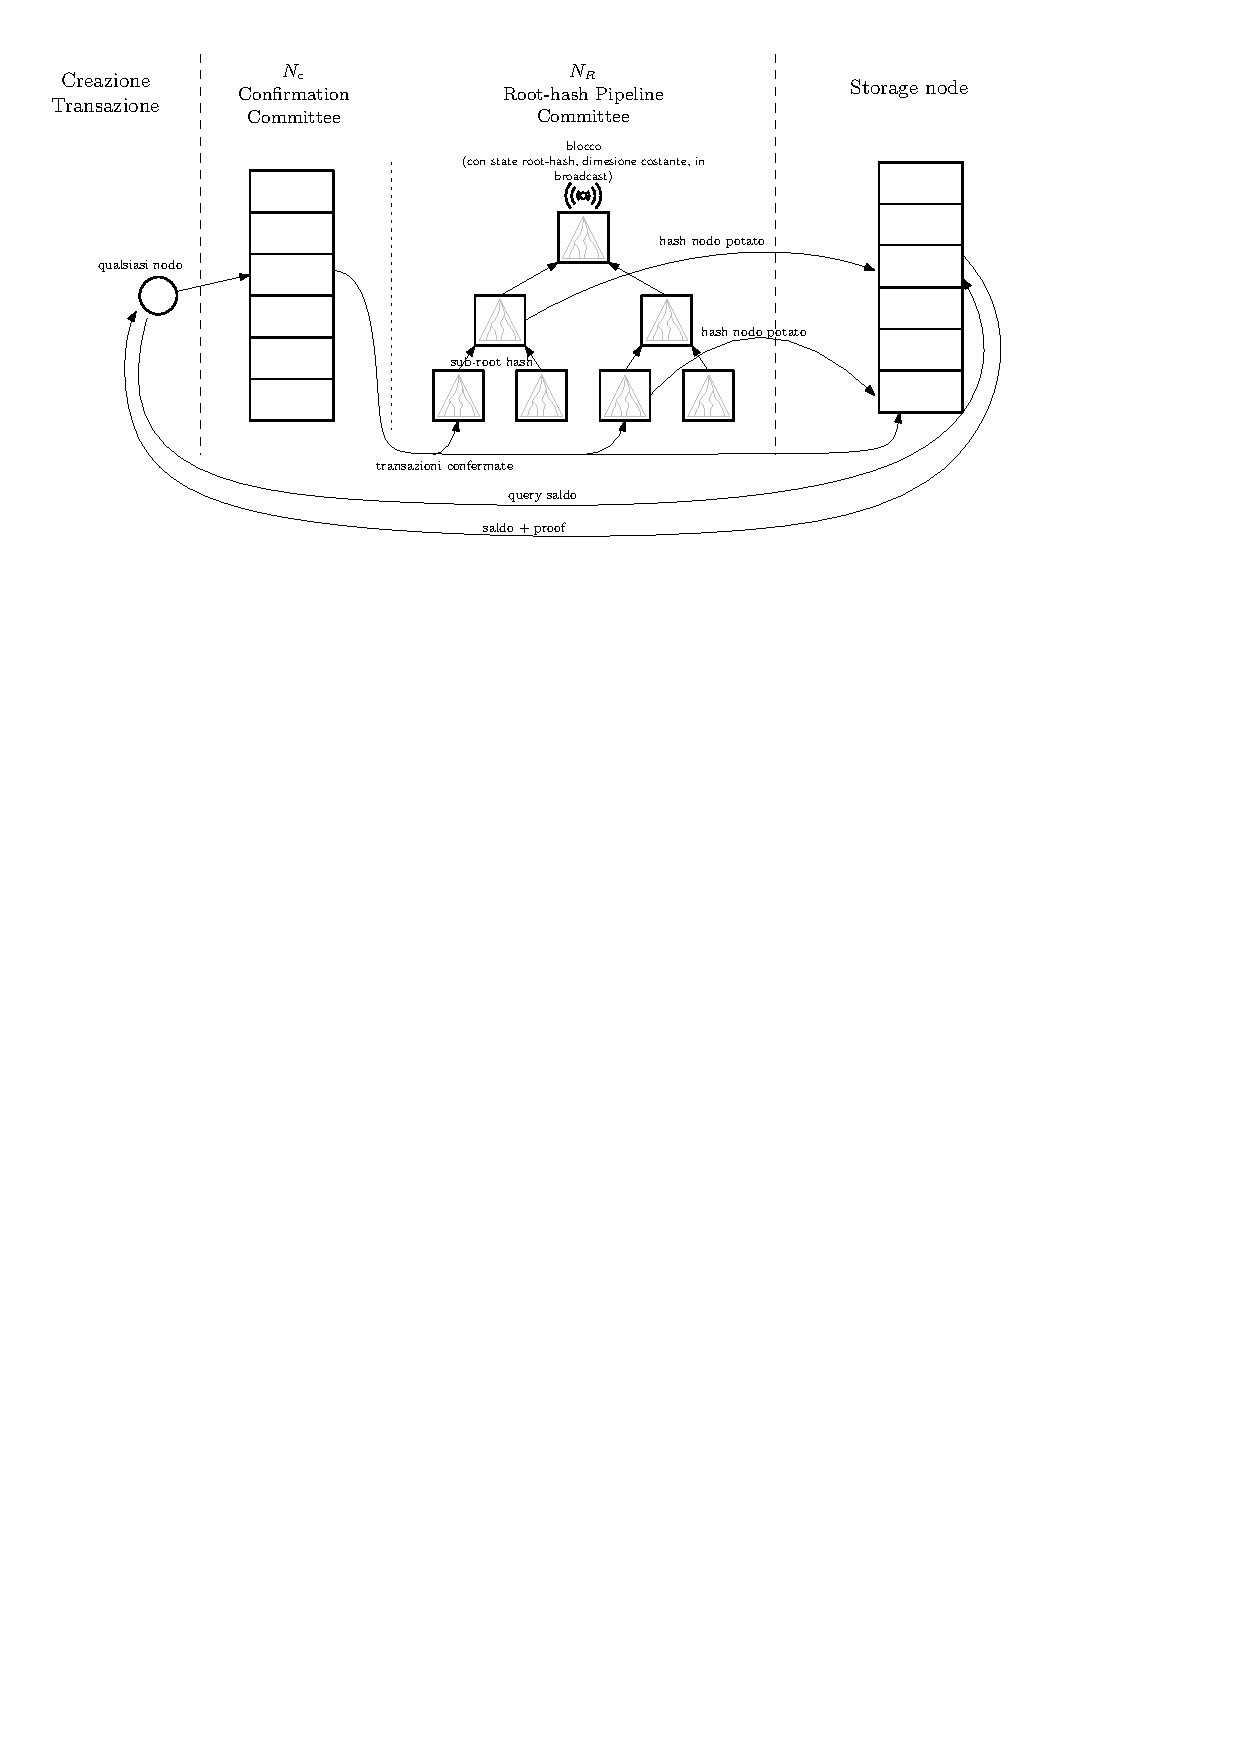
\includegraphics[scale=0.82]{img/captre/bc.pdf}
	\caption{Flusso delle informazioni dell'architettura proposta.}
	\label{fig:architecture}
\end{figure}

Ogni nodo può creare una transazione. Come descritto nel paragrafo precedente, una nuova transazione deve contenere il saldo dei conti associati e le proof di integrità relative, ottenute durante il round precedente dagli storage node autorità per gli elementi di stato coinvolti nella transazione. Le nuove transazioni (candidate) non sono inviate in broadcast come nelle soluzioni tradizionali, ma ad un ristretto numero di nodi.

Il ruolo di validazione e conferma delle nuove transazioni è eseguito dai \emph{Confirmation Committee} (\emph{CC}). Ogni CC è denotato con $C_k$, con $k = 1, \dots, N_c$, dove $N_c$ è il numero di CC. Quando è importante, si denota con $C_k^i$ il $k$-esimo Confirmation Committee relativo al round $i$. Come detto prima, per motivi di sicurezza, ogni Confirmation Committee tra un round e l'altro è formato da membri differenti. Il nodo che crea la transazione $t$, la invia a $C_k^i$ tale che $k = hash(t_s) \mod N_c$, dove $t_s$ è la sorgente della transazione $t$, e si dice che $C_k^i$ è \emph{responsabile} per $t$. Ogni nuova transazione $t$ è ricevuta da $C_k^i$ \emph{prima} del round dell'inizio del round $i$, in modo tale che $C_k^i$ possa processare $t$ durante il round $i$. L'insieme di transazioni per cui $C_k^i$ è responsabile è denotato $P(C_k^i)$. Si denota con $P^i = \cup_k P(C_k^i)$ l'insieme di tutte le transazioni processate da tutti i Confirmation Committee nel round $i$. Il risultato di un $C_k^i$ è una lista di transazioni validate e confermate denotato $A_k^i$, con $A_k^i \subseteq P(C_k^i)$.

$C_k^i$, affinché possa validare correttamente le transazioni, per ogni transazione $t$ ottiene il saldo associato a $B^{i-1}$, in modo da verificare che $t_s$ non diventi negativo applicando la transazione $t$. Poiché le proof fornite in $t$ sono relative a $B_{i-2} = B^{i-q-1}$, esse sono troppo vecchie. Infatti, i conti associati potrebbero essere stati modificati negli ultimi $q$ round, i cui blocchi non sono ancora disponibili (perché la loro creazione è ancora in corso dalla pipeline). Quindi, ogni $C_k^i$ deve conoscere le transazioni confermate, e quindi i cambiamenti allo stato, dai Confirmation Committee dei round precedenti $C_k^{i-q}, \dots, C_k^{i-1}$, ovvero $A_k^{i-q}, \dots, A_k^{i-1}$. Queste transazioni devono essere utilizzate per aggiornare tutti i conti associati alle transazioni in $P(C_k^i)$ per ottenere lo stato di $B^{i-1}$. Questo processo è chiamato \emph{time-updating}.

Ogni $C_k^i$ esegue il seguente algoritmo, tramite un protocollo di consenso:

\paragraph*{Algoritmo 1 (Comportamento dei Confirmation Committee)}\todo{cambiare stile scrittura}
\begin{enumerate}
	\item Verifica che ogni transazione in $P(C_k^i)$ rispetti le regole sintattiche e le proof non sono scadute. Non accetta le transazioni che non passano queste verifiche, generando $P'(C_k^i) \subseteq P(C_k^i)$.
	\item Seleziona una permutazione $\bar{T}$ di $P'(C_k^i)$.
	\item Sia $\widetilde{T}$ la concatenazione di $A_k^{i-q}, \dots, A_k^{i-1}$. Per ogni sorgente nelle transazioni in $\bar{T}$, considera l'ultimo saldo tra i conti delle transazioni in $\widetilde{T}$ e i conti forniti dalle proof delle transazioni in $\bar{T}$.
	\item Esegui le transazioni in $\bar{T}$ e verifica che il saldo risultante di ogni transazione non scenda sotto-zero. Le transazioni che non rispettano questa regola sono scartate. Il risultato è la lista $A_k^i$ ottenuto da $\bar{T}$ dove le transazioni scartate sono omesse.	
\end{enumerate}

Le transazioni in $A_k^i$ si considerano \emph{confermate} e saranno inserite nel blocco $B_i$. Per permettere ai Confirmation Committee dei round successivi di effettuare il time-updating, $C_k^i$ invia $A_k^i$ a $C_k^{i+1}, \dots, C_k^{i+q}$ ed anche ad altri comitati, come mostrato in seguito.

La lista delle transazioni confermate nel round $i$ è denotato $A^i = \cup_k A_k^i$, e rispetta lo stesso ordine delle transazioni in ogni $A_k^i$. Le transazioni in $A_k^i$ sono inviate anche agli storage node, anche se il blocco $B^i$ non è stato ancora creato.

La creazione del blocco $B^i = B_{i+-1}$ richiede il calcolo dello state root-hash. Esso si ottiene dal root-hash del Merkle Tree $W$ relativo all'intero spazio dello stato, che richiede il calcolo di tutti gli hash dei nodi di $W$.
Questo è eseguito da $N_r$ comitati, denominati \emph{Root-hash Pipeline Committee}, o \emph{RPC}. Ad ogni RPC è associato una parte di $W$, denominato \emph{albero sotteso} all'RPC. Gli RPC sono disposti ad albero, denominato \emph{albero degli RPC}, come rappresentato nella Figura~\ref{fig:rpc_tree}\todo{fare figura alberi RPC}. Ogni RPC ha il compito di calcolare gli hash del proprio albero sotteso durante il proprio round. Esistono due tipi di RPC: (1) gli RPC \emph{foglie}, che sono gli RPC disposti come foglie dell'albero degli RPC, e (2) gli RPC \emph{interni}, ovvero tutti gli altri. Ogni RPC foglia è responsabile di un intervallo contiguo dello spazio degli indirizzi che rappresenta le foglie di $W$. Si dice che un RPC è autorità per questo intervallo di indirizzi. Poiché solo una parte dello stato è modificato dalle nuove transazione, gli RPC foglie operano su un albero sotteso che è potato. Questo albero ha per foglie solo gli elementi di stato per cui l'RPC è autorità e che sono stati modificati dalle transazioni nel round corrente. Gli alberi sottesi degli RPC interni sono invece alberi binari completi. Gli RPC sono divisi in \emph{livelli}, numerati da $1$ ad $h$. Gli RPC foglie si trovano al livello 1, mentre a livello $h$ è presente l'unico RPC, radice dell'albero degli RPC. Ad ogni livello corrisponde uno stadio della pipeline. Quindi il numero totale di stadi è $q = h+1$. Ogni albero sotteso ad un RPC ha per radice un nodo, denominato \emph{sub root-hash}. Tutti gli RPC a livello $i < h$ calcolano il proprio \emph{sub root-hash} e lo inviano ai propri genitori nell'albero degli RPC. L'RPC radice dell'albero degli RPC crea il blocco contenente lo state root-hash per il round corrente e lo invia in broadcast a tutti i nodi della rete.

Il generico RPC foglia del round $i+1$ ed autorità dell'$m$-esima porzione dello spazio degli indirizzi è denotato con $R_m^{i+1}$. Gli RPC foglie si trovano al secondo stadio della pipeline, per cui ricevono come input $A_i$, che è l'output dei Confirmation Committee del primo stadio. Tuttavia ogni RPC foglia non ha bisogno di tutte le transazioni in $A_i$, ma solo quelle che coinvolgono gli indirizzi per cui l'RPC è autorità. Se $t$ è una transazione in $A_k^i$, $C_k^i$ invia la transazione ad $R_m^{i+1}$ solo se la sorgente o la destinazione di $t$ è un indirizzo per cui $R_m^{i+1}$ è autorità. Ogni Confirmation Committee invia ogni transazione a due RPC foglie. Si denota con $S_m(A^i) \subseteq A^i$ l'insieme di transazioni che coinvolgono indirizzi che ricadono nell'intervallo $m$ e che sono ricevuti da $R_m^{i+1}$. Ogni $R_m^{i+1}$ ha il compito di calcolare il sub root-hash del proprio albero sotteso relativo al blocco $B^i$. Per questo è necessario lo stato dell'albero sotteso relativo al blocco $B^{i-1}$. Poiché le proof fornite in $S_m(A^i)$ sono relative al blocco $B_{i-2} = B^{i-q-1}$, non possono essere utilizzate da sole per il calcolo degli hash dell'albero sotteso relativo a $B^{i-1}$. Infatti gli indirizzi associati potrebbero esser stati aggiornati dalle transazioni in $A^{i-q}, \dots, A^{i-1}$ per i quali i blocchi corrispondenti non sono ancora disponibili. Quindi, ogni $R_m^{i+1}$ deve conoscere $S_m(A^{i-q}), \dots, S_m(A^{i-1})$. $R_m^{i+1}$ utilizza tutte le proof in $A^{i-q}, \dots, A^{i}$ per calcolare gli hash del proprio albero sotteso, come descritto nel Paragrafo~\ref{sec:bernardini}. Questo processo è chiamato \emph{time-shifting}. Per permettere agli RPC foglie dei successivi round di svolgere il proprio compito, ogni $C_k^i$ invia $S_m(A_k^i)$ a $R_m^{i+1}, \dots, R_m^{i+q+1}$.

Mentre gli RPC foglie hanno bisogno di uno stato per poter effettuare il time-shifting, gli RPC interni sono stateless. Essendo l'albero sottostante completo, hanno bisogno solamente dei sub root-hash calcolati dagli RPC figli nell'albero degli RPC, che corrispondono agli hash delle foglie dell'albero sottostante dell'RPC interno.

Ogni storage node $n$ che memorizza la potatura di $W$, le cui foglie sono gli indirizzi per cui $n$ è autorità, non può calcolarsi direttamente gli hash dei sottoalberi potati. Quindi, durante il calcolo di $W$ relativo al blocco $B^i$, gli RPC inviano questi hash ai nodi che ne hanno bisogno. Questo può essere realizzato in maniera del tutto trasparente agli RPC, creando un canale \textit{publish/subscribe}~\cite{eugster2003many}, a cui gli storage node interessati per un sottoinsieme di nodi potati si iscrivono.

\section{Teorema di correttezza}

In questo paragrafo si dimostra formalmente la correttezza dell'architettura riportata nel Paragrafo~\ref{sec:architettura}.

\begin{lemma}{(Correttezza dell'algoritmo di conferma).}\label{lemma:cc}
L'Algoritmo 1 non restituisce mai una sequenza le cui transazioni comportano una violazione del vincolo del saldo non-negativo.
\end{lemma}

\begin{proof}
Per costruzione dello step 4 dell'Algoritmo 1.
\end{proof}


\begin{theorem}{(Correttezza).}
Sia $P^i$ un insieme di transazioni processate, nel round $i$, dai Confirmation Commitee $C_k^i$ e sia $A_k^i$ la lista delle transazioni confermate da ogni $C_k^i$. Le seguenti affermazioni sono vere.

\begin{enumerate}
	\item In ogni lista $A^i = \cup_k A_k^i$ tale che $A^i$ preserva l'ordine delle transazioni contenute in ogni $A_k^i$, la regola del saldo non-negativo è rispettata.
	\item Lo state root-hash di $B^i = B_{i+q-1}$ è il root-hash del nuovo stato ottenuto dopo l'applicazione delle transazioni in $A^i$.
	\item Gli storage node conoscono le proof degli indirizzi per cui sono autorità.
\end{enumerate}

\end{theorem}


\begin{proof}
Riguardo l'affermazione 1, per il Lemma~\ref{lemma:cc}, $A_k^i$ soddisfa il vincolo del saldo non-negativo e per ipotesi l'ordine delle transazioni in $A^i$ è preservato. Poiché per ogni $k$ gli indirizzi modificati in $A_k^i$ non sono modificati in nessun $A_j^i$ con $j \neq k$, segue l'affermazione.

Riguardo l'affermazione 2, si noti che ogni RPC foglia $R_m^{i+1}$ considera tutte le transazioni in $S_m(A^{i-1}), \dots, S_m(A^{i-1})$, che riguardano gli indirizzi per cui $R_m^{i+1}$ è responsabile, rispettando il loro ordine. Ogni $R_m^{i+1}$ può calcolare correttamente il proprio sub root-hash e passarlo al proprio RPC genitore. Infatti, se un nodo interno nell'albero sotteso è coinvolto in una transazione, $R_m^{i+1}$ riceve le proof della transazione stessa. Se un nodo interno dell'albero sotteso non è coinvolto in alcuna transazione o è potato o è la radice di un sottoalbero potato. Nel primo caso, $R_m^{i+1}$ non ne ha bisogno. Nel secondo, $R_m^{i+1}$ riceve l'hash da una delle proof presenti in $S_m(A^{i-1}), \dots, S_m(A^{i-1})$. Infine, ogni RPC interno, riceve dai propri RPC figli, gli hash delle foglie dei proprio albero sotteso, per cui il calcolo del sub root-hash è banale. Segue quindi l'affermazione.

Riguardo l'affermazione 3, si noti che gli RPC calcolano il root-hash della versione potata $W'$ di $W$, in cui le foglie di $W'$ sono tutti gli indirizzi $U$. Ogni storage node $n$ memorizza una versione potata $W_n$ di $W$, in cui le foglie di $W_n$ sono tutti gli indirizzi $U_n$ che $n$ memorizza. Poiché $U_n \subseteq U$, anche $W_n \subseteq W'$. Quindi, tutti i sub root-hash dei sottoalberi potati di $W_n$ sono conosciuti da uno degli RPC, il qualche può inviarlo ad $n$.
\end{proof}


\section{Teorema di scalabilità}

In questo paragrafo, si dimostra formalmente la scalabilità dell'architettura. Si assume, per semplicità, che i saldi modificati durante un round siano uniformemente distribuiti sullo spazio degli indirizzi.
Sia $f$ la frequenza delle transazioni che arrivano alla blockchain. Sia $\Delta$ la durata di un round. Sia $m = 2 f \Delta$ il numero di indirizzi il cui saldo viene modificato in un round, assumendo che le transazioni coinvolgano indirizzi distinti. Sia $\widetilde{W}$ la versione di $W$ potata che ha solo $m$ foglie, quelle il cui saldo è modificato in un round. Esiste un livello $l$ di $\widetilde{W}$ al disopra del quale $\widetilde{W}$ è un albero binario completo. Più $m$ è grande, più la parte potata diventa più piccola ed $l$ si avvicina alle foglie.

Sia $j$ il massimo numero di hash che un RPC può calcolare in un round. Si noti che $j$ è constante, poiché dipende dalla capacità computazionale dei nodi di un comitato. Sia $e$ il massimo numero di indirizzi il cui saldo viene modificato che un RPC foglia $R$ sia in grado di processare in un round. Ovviamente $e$ dipende da $j$ e come sono distribuiti gli indirizzi nello spazio degli indirizzi di cui $R$ è autorità. Tuttavia, per ipotesi gli indirizzi modificati sono uniformemente distribuiti, per cui $e$ è uguale per tutti gli RPC foglia. Si assume che $j$ sia grande abbastanza in modo che la radice dell'albero sottostante ad un RPC foglia sia sopra il livello $l$. Quindi, l'albero sottostante $U$ di un RPC interno $R$ è binario e completo. Sia $k$ l'altezza di $U$. Il numero di nodi di $U$ è $2^k-1$. Gli RPC figli di $R$ sono $2^{k-1}$. In ogni round, ogni RPC deve calcolare un hash per ogni nodo del proprio albero sottostante $U$. Il massimo numero di nodi in un albero sottostante ad un RPC interno è $\hat{j} = 2^{\hat{k}}-1$, dove $\hat{k}$ è il più grande numero intero tale che $\hat{j} \leq j$, o in maniera equivalente $\hat{k} = \floor*{\log_2 (j+1)}$. L'altezza massima di un di un albero sottostante ad un RPC è $\hat{k}$.

Sia $S(N, f)$ un sistema di blockchain, avente un'architettura descritta nel Paragrafo~\ref{sec:architettura}, con $N$ nodi ed un carico di frequenza $f$.

\begin{lemma}\label{lemma:rpc_count}
Sia $S(N, f)$ una blockchain, di $N$ nodi con un carico di frequenza $f$. Sia $e$ il massimo numero di indirizzi il cui saldo è stato modificato che un RPC foglia può processare in un round, e $\hat{j}$ il massimo numero di hash che un RPC interno può calcolare in un round. Se $S$ è ben dimensionato, il numero di RPC foglie è almeno $2^{\ceil*{\log_2 (m/e)}}$ ed il numero di RPC interni è almeno $\ceil*{\frac{2^{\ceil*{\log_2 (m/e)} - 1}}{\hat{j}}}$, in cui $m = 2 f \Delta$ e $\Delta$ è la durata di un round.
\end{lemma}

\begin{proof}
Gli RPC foglie sono almeno $\ceil*{m/e}$ e poiché sono le foglie di un albero completo, il loro numero è una potenza di 2. Quindi devono essere $2^g$ con $g = \ceil*{\log_e (m/e)}$.

Quando $m$ aumenta, il numero di risorse usate in ogni RPC foglia aumenta. Quando le risorse di un RPC foglia sono sature, il loro numero raddoppia. Immediatamente dopo un raddoppio, le loro risorse sono utilizzate a metà. Aumentando $m$, le risorse utilizzate vanno da $m$ alla massima capacità computazionale, che si ha subito prima di un raddoppio.

Si consideri l'albero composto dagli RPC interni $W_I$, la sua altezza è $g$. Poiché gli RPC foglia sono $2^g$, i nodi di $W_I$ sono $2^g -1$. Quindi il numero di RPC interni è $\ceil*{\frac{2^g-1}{\hat{j}}}$.
Da notare che sia il numeratore che il denominatore rappresentano la dimensione di un albero binario completo, con altezza $g$ e $\hat{k}$, rispettivamente. La parte intera del risultato della divisione rappresenta il numero di RPC interni con una dimensione dell'albero sottostante pari a $\hat{j}$. Il resto  è la dimensione della radice dell'albero degli RPC che è in generale sottodimensionato, rispetto alla sua potenza computazionale.
\end{proof}


\begin{theorem}{(Scalabilità).}\label{th:scalability}
Sia $S(N, f)$ una blockchain well-provisioned composta da $N$ nodi ed un carico di frequenza $f$. Per ogni $\alpha > 1$ tale che $a N$ è intero, la blockchain $\bar{S}(\alpha N, \alpha f)$ è well-provisioned, supponendo un carico uniformemente distribuito sullo spazio degli indirizzi.
\end{theorem}

\begin{proof}
Sia $S(N, f)$ un sistema well-provisioned immediatamente dopo un raddoppio, ovvero con gli RPC foglie al minimo delle risorse computazionali utilizzate. In $S$ e in $\bar{S}$ i comitati hanno la stessa potenza computazionale. Si vuole mostrare che $\alpha N$ nodi sono sufficienti per formare dei comitati in grado di processare in carico $\alpha f$.

Un carico di frequenza $f$, genera un numero di transazioni $f \Delta$ per round. Sia $N_C$ il numero di Confirmation Committee in $S$. Poiché, per ipotesi, $S$ è well-provisioned, ogni CC è in grado di processare $f \Delta / N_C$ transazioni per round. In $\bar{S}$ il carico è $\alpha f$, quindi, con $\alpha N_C$ CC, si ha che ogni CC in $\bar{S}$ processa lo stesso numero di transazioni che in $S$.

Si utilizzano i simboli $m$, $e$, $\hat{j}$ e $g$ con lo stesso significato di prima.
Subito dopo un raddoppio, $m/e$ è una potenza di 2, $g= \log_2 (m/e) +1$, per il Lemma~\ref{lemma:rpc_count} il numero di RPC in $S$ è $N_R = 2^g + \ceil*{2^g/\hat{j}} = 2m/e + \ceil*{2 m/ (e \hat{j}}$. Si considera ora il numero di RPC $\bar{N_R}$ necessari in $\bar{S}(\alpha N, \alpha f)$. Per $\alpha = 2^t$ con $t$ positivo ed intero, $\bar{N_R} = 2 \alpha m / e + \ceil*{2 \alpha m / (e \hat{j})}$. Poiché $\ceil{2 \alpha m/(e \hat{j}} \leq \alpha \ceil*{2 m / (e \hat{j}}$, $N_R \leq \alpha N_R$.

Quindi, l'incremento richiesto da $\bar{S}$ a partire da $S$ del numero di CC ed RPC è al massimo di un fattore $\alpha$ e $\bar{S}$ ha $\alpha N$ nodi. Quindi $\bar{S}$ è well-provisioned.
\end{proof}


\section{Comunicazione inter-committee}

Nel paragrafo precedente, nella descrizione dell'architettura, si è citata una forma di comunicazione tra comitati, o \emph{comunicazione inter-committee}, in modo che un comitato possa inviare dei dati ad un altro comitato del round successivo, oppure un nodo possa inviare la transazione candidata al CC responsabile.
Un nodo non comunica con un comitato in unicast. Questo richiederebbe infatti la conoscenza di tutti le destinazioni, che è un problema di scalabilità considerando che i membri di ogni comitato cambiano ad ogni round. Un approccio basato su multicast può essere invece una soluzione, non utilizzando approcci tradizionali, come~\todo{citazione a pim sparse mode}, che poco si adattano alle specifiche richieste dall'architettura.

In seguito è presentata un'analisi delle specifiche di ogni comunicazione multicast. Sia $N$ il numero dei nodi nella rete. Siano $N_C$, $N_R$, $e$, $m$, $\hat{j}$ e $q$ variabili con lo stesso significato dei precedenti paragrafi.
Sia $n_{cr}$ un nodo generico nodo della rete che crea una transazione candidata. Sia $S$ la dimensione dello spazio degli indirizzi. Sia $R^i$ un Root-hash Pipeline Committee nel round $i$.

Sono stati individuati cinque flussi multicast, riportati nella Tabella~\ref{tab:multicast}.

\begin{sidewaystable}
\centering
\begin{tabular}{c|c|c|c|}
\cline{2-4}
                                                                      & \textbf{Gruppi multicast}               & \textbf{Subscriber}                                                                                                                        & \textbf{Publisher}                                  \\ \hline
\multicolumn{1}{|c|}{$n_{cr} \rightarrow C_k$}                        & $N_C$                          & $\dfrac{N}{N_C + N_R}$                                                                                                            & $O(N)$                                       \\ \hline
\multicolumn{1}{|c|}{$C_k^i \rightarrow R_m^{i+1}$}                   & $\ceil*{m/e}$                  & $\dfrac{N}{N_C + N_R}$                                                                                                            & $\dfrac{N_C N}{N_C + N_R} = O(N)$          \\ \hline
\multicolumn{1}{|c|}{$R^i \rightarrow R^{i+1}$}                       & $\dfrac{\hat{j}+1}{2}^{h-i-1}$ & $\dfrac{N}{N_C + N_R}$                                                                                                            & $\dfrac{\hat{j}+1}{2}\dfrac{N}{N_C + N_R}$ \\ \hline
\multicolumn{1}{|c|}{$C_k \rightarrow DHT$}                           & S                              & \begin{tabular}[c]{@{}c@{}}ciascuno storage node\\ si iscrive ai gruppi\\ relativi agli elementi\\ di cui è autorità\end{tabular} & $\dfrac{N}{N_C + N_R}$                     \\ \hline
\multicolumn{1}{|c|}{$C_k^i \rightarrow C_k^{i+1}, \dots, C_k^{i+q}$} & $q N_C$                        & $\dfrac{N}{N_C + N_R}$                                                                                                            & $\dfrac{q N}{N_C + N_R}$                   \\ \hline
\multicolumn{1}{|c|}{$R^i \rightarrow DHT$}                           & S                              & \begin{tabular}[c]{@{}c@{}}ciascuno storage node\\ si iscrive ai gruppi\\ relativi agli elementi\\ di cui è autorità\end{tabular} & $\dfrac{N}{N_C + N_R}$                     \\ \hline
\end{tabular}
\caption{Specifiche di ogni flusso multicast.}
\label{tab:multicast}
\end{sidewaystable}


In particolare, si devono tenere in considerazione i seguenti aspetti per il multicast nella comunicazione tra comitati oppure per inviare una transazione candidata al CC autorità:

\begin{itemize}
	\item I membri di un comitato cambiano frequentemente, ad ogni round;
	\item I gruppi multicast devono essere pronti in anticipo rispetto a quando devono essere effettivamente utilizzati;
	\item I gruppi multicast sono necessari solo per un round.
\end{itemize}

Il problema della realizzazione di un multicast che rispetti queste specifiche rimane un problema aperto.

L'ultimo aspetto, una volta realizzata la comunicazione multicast, riguarda l'accettazione di un messaggio da parte di un comitato $C_{out}$ ricevuto dal comitato $C_{in}$. Infatti, $C_{in}$ potrebbe essere composto da nodi malevoli, che possono o decidere di non inviare il messaggio o di cambiarne il contenuto.
Un comitato $C_{out}$ interessato a ricevere messaggi da parte di comitato $C_{in}$, si iscrive ad un gruppo multicast come subscriber. $C_{in}$ invia i messaggi come publisher del gruppo multicast. Ogni membro del comitato $C_{in}$ invia lo stesso messaggio, che è ricevuto da ogni membro di $C_{out}$. $C_{out}$ accetta un messaggio $m$ da $C_{in}$ solo se $m$ è stato inviato da più della metà dei membri di $C_{in}$.

\section{Discussione}

In questo paragrafo si discute l'effettiva risoluzione del blockchain scalability trilemma, cercando di capire se la scalabilità limiti la decentralizzazione e/o la sicurezza, come in altri approcci presenti in letteratura.
Riguardo la \textit{decentralizzazione}, anche se ogni nodo della rete ha un ruolo diverso nella creazione del blocco, i membri ad ogni comitato sono assegnati e cambiati periodicamente in modo randomico, come in~\cite{gilad2017algorand}.
I ruoli sono quindi statisticamente omogenei. Quindi la scalabilità non impatta la decentralizzazione.

Riguardo la \textit{sicurezza}, il Teorema~\ref{th:scalability} mostra come la scalabilità non riduce la dimensione di ogni singolo comitato. Molti attacchi, come quelli presentati nel Paragrafo~\ref{attacks}, richiedono che l'attaccante controlli la maggior parte dei nodi di un comitato. Tuttavia, quando i membri di un comitato sono selezionati in modo randomico, l'attacco è molto più difficile. Inoltre, utilizzando approcci basati su Proof-of-Stake, ed in generale protocolli di consenso distribuito robusti, si evitano attacchi Sybil. Quindi la scalabilità non ha impatto sulla sicurezza.
